\documentclass[tikz,border=2pt]{standalone}
\usepackage{amsmath}
\usetikzlibrary{arrows.meta}
\begin{document}
% x = (3, 1, 4, 2, 5, NA): x == NA is NA everywhere, x == "NA" is FALSE except NA at the gap,
% is.na(x) is FALSE except TRUE at the gap.
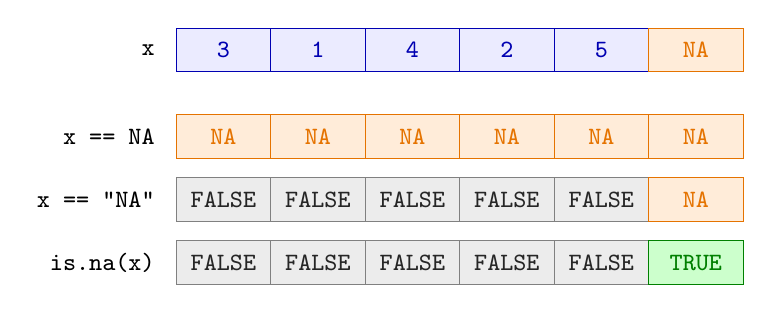
\begin{tikzpicture}[font=\small, >={Latex[length=2mm]},
  cell/.style={draw, minimum width=1.2cm, minimum height=0.55cm, inner sep=1pt, font=\small\ttfamily},
  val/.style={cell, draw=blue!70!black, fill=blue!8, text=blue!70!black},
  yes/.style={cell, draw=green!50!black, fill=green!20, text=green!50!black},
  no/.style={cell, draw=gray, fill=gray!15, text=gray!30!black},
  na/.style={cell, draw=orange!90!black, fill=orange!15, text=orange!90!black},
  lab/.style={anchor=east, font=\small\ttfamily}]
  \node[lab] at (0.45,0) {x};
  \foreach \s/\t [count=\i] in {val/3,val/1,val/4,val/2,val/5,na/NA} { \node[\s] at (1.2*\i,0) {\t}; }
  \node[lab] at (0.45,-1.1) {x == NA};
  \foreach \i in {1,...,6} { \node[na] at (1.2*\i,-1.1) {NA}; }
  \node[lab] at (0.45,-1.9) {x == "NA"};
  \foreach \s/\t [count=\i] in {no/FALSE,no/FALSE,no/FALSE,no/FALSE,no/FALSE,na/NA} { \node[\s] at (1.2*\i,-1.9) {\t}; }
  \node[lab] at (0.45,-2.7) {is.na(x)};
  \foreach \s/\t [count=\i] in {no/FALSE,no/FALSE,no/FALSE,no/FALSE,no/FALSE,yes/TRUE} { \node[\s] at (1.2*\i,-2.7) {\t}; }
\end{tikzpicture}
\end{document}
